\documentclass{acm_proc_article-sp}
\usepackage{caption,subcaption}
\usepackage[ruled, vlined]{algorithm2e}

\begin{document}

\title{Using Information Theoretic Criteria to Discover Useful Options}


\numberofauthors{2} %  in this sample file, there are a *total*
% of EIGHT authors. SIX appear on the 'first-page' (for formatting
% reasons) and the remaining two appear in the \additionalauthors section.
%
\author{
% 1st. author
\alignauthor
Viktoria Kovecses\\
       \affaddr{McGill University}\\
       \email{viktoria.kovecses@mail.mcgill.ca}
% 2nd. author
\alignauthor
Doina Precup\\
       \affaddr{McGill University}\\
       \email{dprecup@cs.mcgill.ca}
}

\maketitle
\begin{abstract}

	Reinforcement learning allows autonomous agents to compute optimal ways of behaving by interacting with an environment. Temporally extended actions, or options, allow algorithms to achieve faster convergence to an optimal policy. While options can be defined manually for some MDPs, this is difficult in general because it may be unclear what options are good without prior knowledge of the environment. Therefore, it is beneficial to find good options automatically. We propose a novel approach which creates random options and then sifts through them using an information theoretic policy search algorithm. The algorithm combines a measure of predictive information and rewards to guide the agent. Our approach shows promising empirical results on small navigation problems and is computationally efficient. 
	
\end{abstract}

% A category with the (minimum) three required fields
%\category{H.4}{Information Systems Applications}{Miscellaneous}
%A category including the fourth, optional field follows...
%\category{D.2.8}{Software Engineering}{Metrics}[complexity measures, performance measures]

%\terms{Theory}

\keywords{finding options, information theory, predictive information} % NOT required for Proceedings

\section{Introduction}

People often use different levels of planning to execute their everyday actions. For instance, the action of making an appointment may consist of many sub-actions, such as picking up the phone, dialling the number, and speaking to the receptionist. The abstraction of sub-actions into larger more compact actions is therefore useful in everyday life. However, it may also be useful in the context of reinforcement learning.

Temporal abstraction of actions has proved to be a useful tool allowing for faster convergence of algorithms to an optimal policy in Markov Decision Processes (MDPs). These temporally abstracted actions are often referred to as options, and they in general consist of a set of states, a policy, and termination conditions. 

Although options may be a very powerful tool once created, they are not always easy to instantiate manually. In some environments the state space may be simply too large, while in others it may not be evident what a good option would consist of. Therefore, it would be beneficial to be able to generate options programmatically for any given environment.

Previous work on finding useful options has shown that for at least some environments it is beneficial to define the option in such a way that the goal state of the subpolicy is a bottleneck (e.g. a hallway between rooms) \cite{solwayoptimal}. However, the methods used require a lot of data to work, and the methodology is involved. Another method for finding options is to look at solutions to several tasks in the same environment, and observe where the optimal actions overlap \cite{pickett2002policyblocks}. The states where the actions remain constant across tasks can then be used to make options. However, this also requires optimally solving several problems before options can be constructed.

In our project, we use a generate-and-test approach instead, in which we create random options and then examine them to determine which are useful using an information theoretic driven policy search algorithm \cite{still}. Essentially, we would like to examine whether using predictive information (i.e. $I[(A_t,X_t); X_{t+1}]$) as well as the return in the environment could be useful in finding decent options for any given MDP.

\section{Background} 

To begin we give a brief overview of reinforcement learning, options, and information theory, as well as important terminology and notation.

\subsection{Reinforcement Learning}

The reinforcement learning framework involves an agent learning about an environment by interacting with it across discrete time steps. To accomplish this the agent moves around by taking different actions, and accumulating rewards as it goes.
	 The environment is often modelled as a Markov Decision Process (MDP) \cite{Puterman}, which consists of a set of states $\mathcal{S}$, a set of actions $\mathcal{A}$, a transition probability matrix $\mathcal{P}$, and a reward function $\mathcal{R}$. Each state represents a portion of the environment, while the actions can be applied to take the agent from one state to another. 
	 The transition probability matrix contains the probability that the agent ends up at state $s_{t+1}$ if it takes action $a_t$ in state $s_t$ at time t. Finally, the reward function indicates the reward $r_{t+1}$ that the agent obtains by taking action $a_t$ in state $s_t$. In addition, the agent may act according to a policy $\pi$, which is a mapping of actions to states that indicates the action to take at each state. The goal of the agent now becomes to maximize the accumulated reward by finding an optimal policy in the environment.  
	 
\subsection{Options}

In many situations it may be beneficial to use temporal abstraction to allow the agent to plan using different levels in the environment. For example, if we want the agent to walk straight until it reaches an obstacle in a continuous environment, we may not want to tell it what to do at each state, but simply give it instructions to move in the same direction for a certain period of time. This would be an example of a temporally abstracted action.

By defining a fixed subpolicy for a group of states in an MDP before the agent begins exploration, one can achieve a faster convergence to an optimal policy. More formally, we may refer to these as options, which are made up of three parts (i.e. $<\mathcal{I}, \pi, \beta>$) : an initiation set $\mathcal{I}$, a policy $\pi$, and termination conditions $\beta$ \cite{sutton1999between}. The initiation set, a subset of the state space, includes all the states where the option can be executed, the policy represents how the agent should act in each of these states, and the termination condition is the probability that the option will terminate at any given state \cite{sutton1999between}.

\subsection{Information Theory Aspect}

In this section we explain a few key concepts of information theory that were an important aspect of the algorithm used in our research.

\subsubsection{Predictive Information}

In information theory mutual information is often defined as the information that a random variable X carries about a random variable Y, and vice versa. In other words, it tells us how well knowing one of the random variables can help us predict the other, and is calculated as follows:

\[I(X; Y) = \sum_{x \in X}\sum_{y \in Y}p(x,y)log(\frac{p(x,y)}{p(x)p(y)})\]

The predictive information is then defined to be the information that the current state and action carry about the state the agent will end up in next (i.e. $I[(A_t,X_t); X_{t+1}]$). It can also be thought of as a measure of the ability of the agent to predict where it will move if it takes an action at its current state. 

\subsubsection{Kullback-Leibler Divergence}

The Kullback-Leibler divergence between two probability distributions is defined as follows: 
\[D_{KL}(p || q) = \sum_{x \in X} p(x)log(\frac{p(x)}{q(x)})\]

It essentially measures the difference between two probability distributions $p$ and $q$. For instance, if the two probability distributions are identical, the divergence would be 0, and if they are very different then the divergence may go to infinity.

In order to maximize the predictive information, as the information theoretic aspect of the algorithm aims to do, we do not directly calculate the predictive information using the mutual information formula, but instead use the Kullback-Leibler divergence between the transition probabilities (i.e. the true model) and the empirically calculated steady state distribution: $D_{KL}(p(X_{t+1}|a, x_t) || p^\pi(X_{t+1}))$. If we consider the steady state distribution $p^\pi(X_{t+1})$ to be an approximation of the transition probability distribution, then we can use the divergence as a measure of the predictive information. For example, if the steady state distribution is very different from the transition probability distribution, then what the agent observes about the environment is not yet close to what the agent expects to see. Therefore, more exploration is required to reduce the divergence and hopefully bring the steady state distribution closer to the transition probability distribution if possible. 

\subsection{Algorithm} 

The algorithm used in our research was taken from previous work completed by Doina Precup and Suzanne Still \cite{still}. It is a policy search algorithm which takes into account both the predictive information in the environment (i.e. $I[(A_t,X_t); X_{t+1}]$), as well as the return, in order to compute an optimal deterministic policy which may be tuned to encourage a certain amount of exploration in the environment. The policy is computed at each time step using the following equation: $$q_{opt}(A_t = a| X_t = x) = \frac{p_t(a)e^{\frac{1}{\lambda}*(D(x,a) + \alpha*Q(x,a))}}{Z(x)}$$ where $D(x,a)$ represents the Kullback-Leibler divergence between the true model and an estimated steady state distribution, or how well the estimated model predicts the true model; and $Q(x,a)$ represents the action values as in usual reinforcement learning (see Algorithm 1).

In order to incorporate options into the algorithm, the options were treated similarly to primitive actions. An option normally takes several time steps to execute; however, here instead we consider the option to execute for only one time step. In essence, we execute the option until termination, but do not make any updates to the policy while the option is running. Instead, once the option terminates, we consider the option to have executed for only one time step, seemingly teleporting from one state to another. However, the action values are updated even as the option is executing, thus providing extra updates for the primitive actions taken within the option, as well as all states in the options initiation set (i.e. all states visited have their action values updated as if the option had been initiated there). 

\begin{algorithm}[h!]
	\SetAlgoLined
	%\DontPrintSemicolon
	 Learn the true model by exploring the environment with a random policy for 1000 trials\;
	 Initialize a uniformly random policy $\pi$\;
	 $Q(x,a) \longleftarrow 0\ \forall x \in X, \forall a \in A \bigcup O$\;
	 $\lambda \longleftarrow 3000$\;
	 \For{each trial i = 0 to 3000}{
		Set starting state\;
		\For{each time step t = 0 to 1000}{
			Get current state $x_{t}$\;
			Update estimate of state visitation distribution as follows:\\
				\Indp $p_{t}(x_{t}) \longleftarrow p_{t}(x_{t}) + 1$\;
				renormalize $p_{t}(x)\ \forall x \in X$\;
			\Indm $q^{(0)}(a|x) \longleftarrow \pi(a|x),\ \forall a \in A \bigcup O, \forall x \in X$\;
			\BlankLine
			\While{$D_{L1}(q^{(j)}, q^{(j+1)}) > 0.5$ and $D_{L1}(q^{(j)}, q^{(j+1)}) < D_{L1}(q^{(j-1)}, q^{(j)})$}{
				\BlankLine
				\BlankLine
				$p^{(j)}(a) \longleftarrow \sum\limits_{x} q^{(j)}(a|x)p_{t}(x),\ \forall a \in A \bigcup O$\;
				$p^{(j)}(x') \longleftarrow \sum\limits_{x} \sum\limits_{a} p(x'|a,x)q^{(j)}(a|x)p_{t}(x)$,\\ \Indp $\forall x' \in X$\;\Indm
				\BlankLine
				$Z^{(j)}(x_{t}) \longleftarrow \sum\limits_{a} p_{t}(a)e^{\frac{1}{\lambda}*(D^{\pi}(x_{t},a) + 10*Q(x_{t},a))}$\;
				\BlankLine
				$q^{(j+1)}(a|x_{t}) \longleftarrow \frac{p^{(j)}(a)}{Z^{(j)}(x_{t})}e^{\frac{1}{\lambda}*(D^{\pi}(x_{t},a) + 10*Q(x_{t},a))},\ \forall a \in A \bigcup O$\;
			}
			$\pi \longleftarrow q^{(j+1)}$\;
			Select next action based on $\pi$ and obtain reward $r_{t+1}$ and next state $x_{t+1}$\;
			Update true model estimates\;
			Update action-value function using Q-learning\;
		}
		$\lambda \longleftarrow 1/log(i+2)$\;
	 }
	 \caption{Pseudocode for policy-search algorithm}
\end{algorithm}

\subsection{Experiments}

Here we give an overview of the environments in which the algorithm was tested.

\subsubsection{Grid Environments}

%add a figure of the grid environment

For the experiments, different variations of a simple 10 x 10 grid world were created. They all contained a start state and a goal state, and the dynamics of the environment remained constant across variations. The agent would always start from the start state and try to move towards the goal which had a reward of +1, while the reward everywhere else was 0. The action space contained four primitive actions which the agent could take, namely $up, down, left$, and $right$; and these actions simply moved the agent towards the corresponding adjacent square. For any primitive action taken, there was a 0.7 probability that the action would succeed, and in the event of failure a different action would be chosen at random. 

%A few of the experiments were also conducted on a 10 x 10 grid world identical to the one previously described, except for this grid world did not contain any obstacles, and therefore had many possible paths from the start to the goal.

%For the majority of experiments, a 10 x 10 grid environment was used (see figure). It contained a start and goal state, as well as obstacles arranged to make two distinct paths between the start and the goal. Though both paths were of equal length, one of the paths (top) was straightforward and made it easy to reach the goal, whereas the other path was winding and less obvious. The agent would always start from the start state and try to move towards the goal which had a reward of +1. The reward everywhere else was 0. The action space contained four primitive actions which the agent could take, namely $up, down, left$, and $right$; and these actions simply moved the agent towards the corresponding adjacent square. For any primitive action taken, there was a 0.7 probability that the action would succeed, and in the event of failure a different action would be chosen randomly. 

\subsubsection{Interesting area}

In order to test whether the information theoretic criteria had any influence in the agent's exploration, an area of interest was added to some of the grid environments. This area consisted of a set of states in which either the reward or the probability of an action succeeding would vary, based on a Gaussian or Uniform probability distribution, respectively. In the case that the reward was varied, the average reward remained 0, and therefore going through this area to reach the goal ultimately made no difference in reward for the agent compared to other paths.

%\subsubsection{Empty Grid World}

\subsection{Results}

Before attempting to remove bad options or chose good options from the environment, a series of experiments were conducted on the grid world environments, mentioned above, in order to determine how the algorithm would choose between both good and bad options and actions, and the nature of the policies that would be produced.

%Giant option
In Figure 1, the algorithm is used on a grid world with a large random option, composed of every state except the subgoal where the option terminates. The policy found (depicted in the right panels) only includes the option if it moves the agent closer to the goal from most states, and leads to improved performance when it is used. This shows the ability of this technique to sift through options and potentially make it easier to find good options without making any assumptions about the environment.

%Giant option
\begin{figure*}[!htbp]
  \begin{subfigure}[h]{.5\textwidth}
  	\centering
    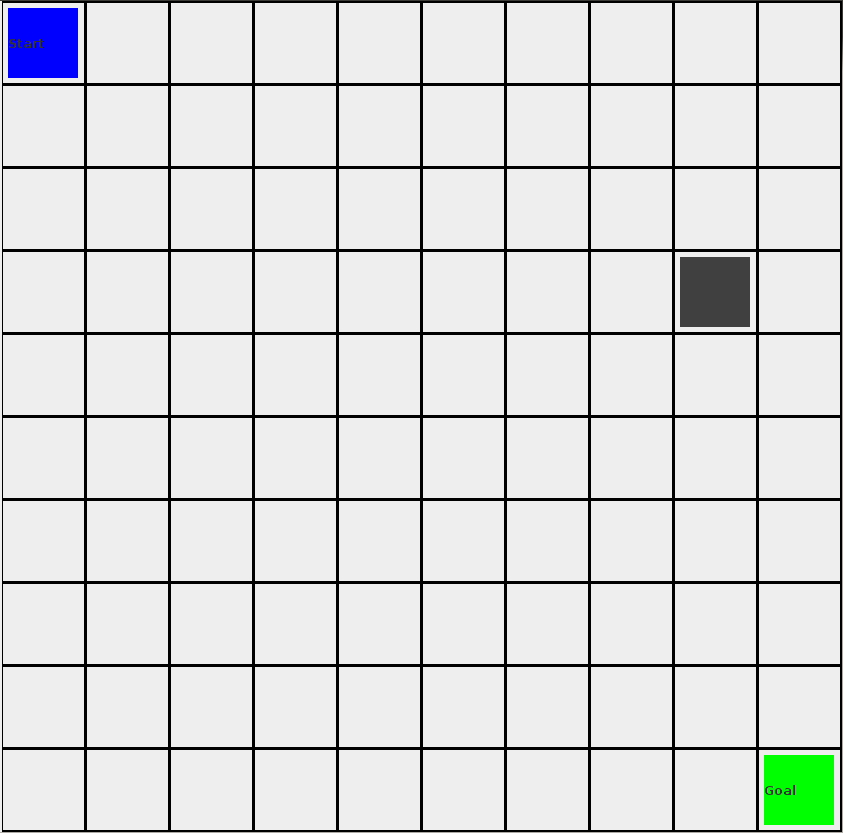
\includegraphics[width=2in]{GiantOp1.png}
    \caption{Option which leads most states away from the goal}
  \end{subfigure}\hfill
  \begin{subfigure}[h]{.5\textwidth}
  \centering
    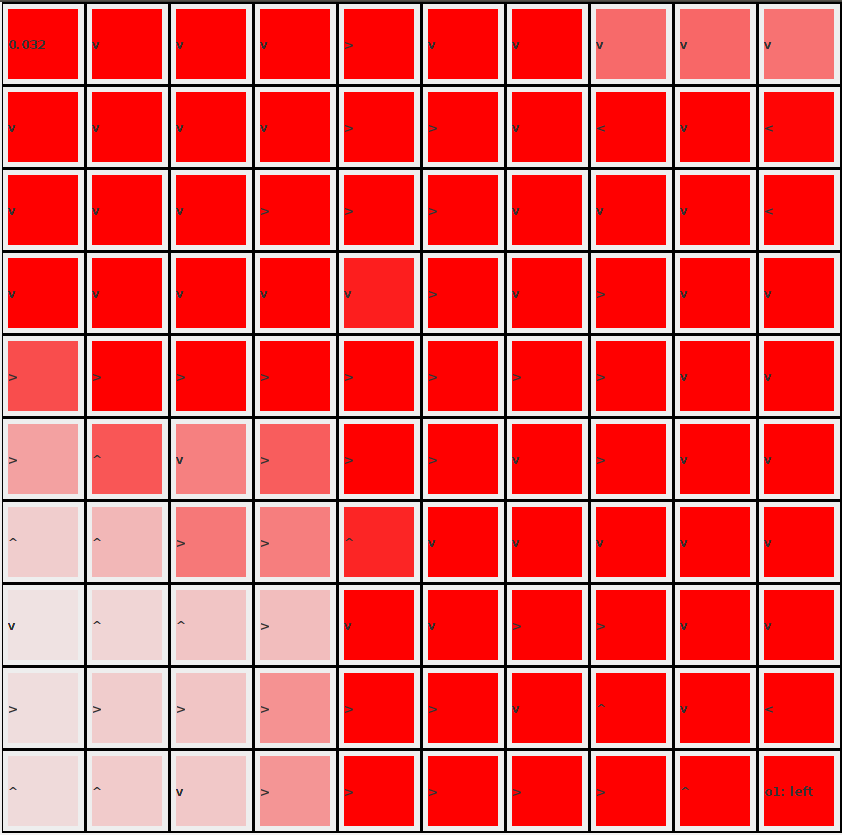
\includegraphics[width=2in]{GiantOption1Pol.png}
    \caption{Option (from (a)) is not selected in any of the states}
  \end{subfigure}
  \hfill
  \begin{subfigure}[h]{.5\textwidth}
  \centering
    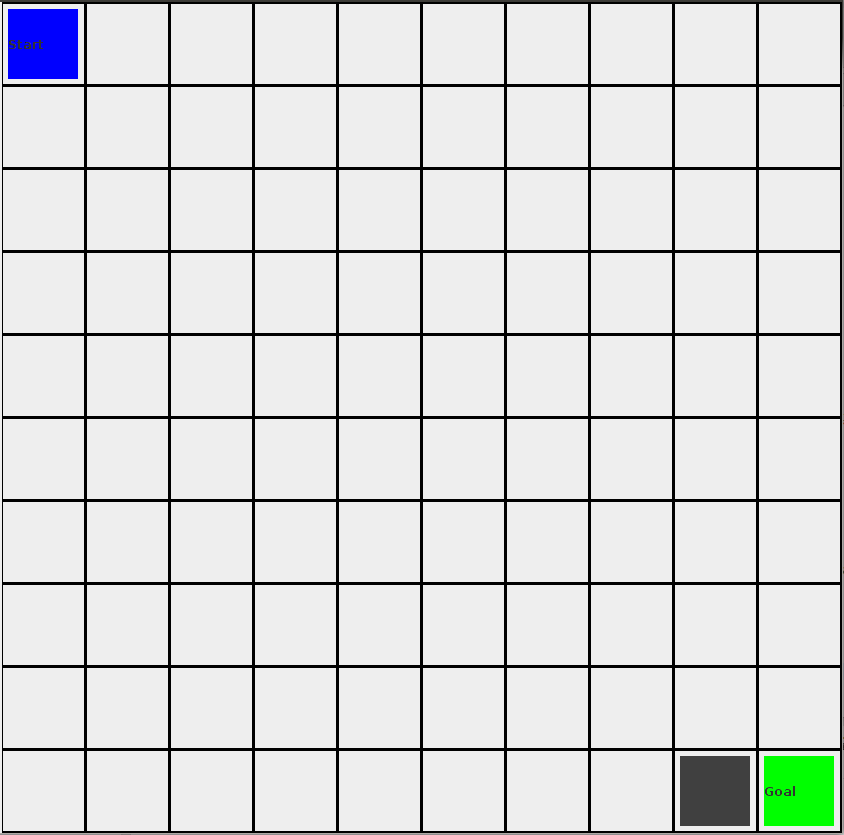
\includegraphics[width=2in]{GiantOp2.png}
    \caption{Option which leads most states towards the goal}
  \end{subfigure}
  \hfill
  \begin{subfigure}[h]{.5\textwidth}
  \centering
    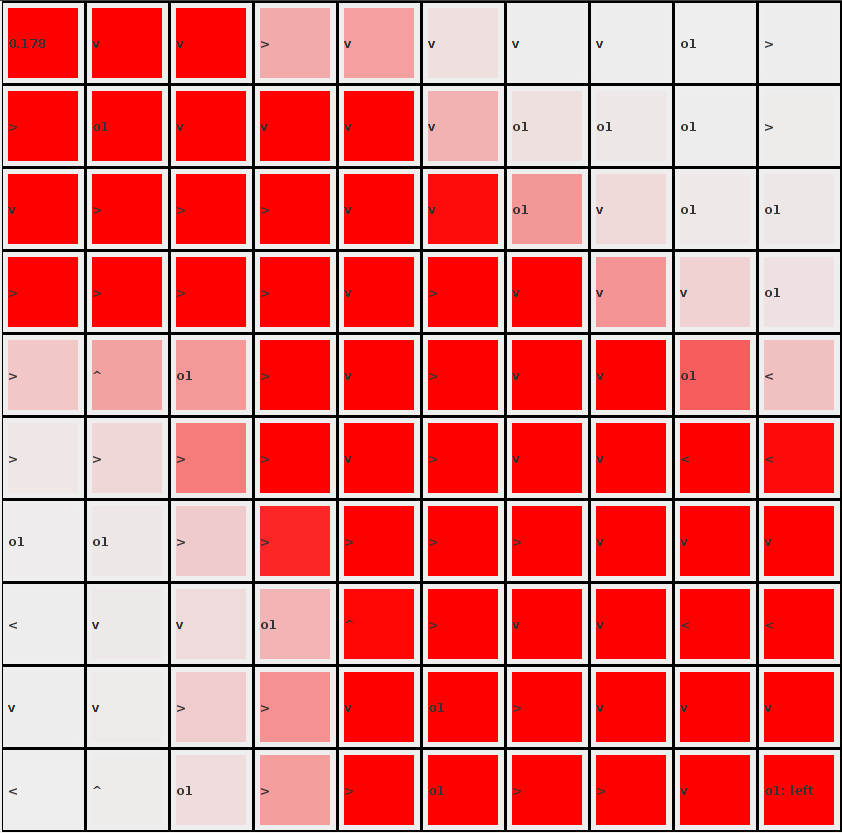
\includegraphics[width=2in]{GiantOp2Pol.png}
    \caption{Option (from (c)) is selected in several states}
  \end{subfigure}
  \caption{Results of testing the algorithm on an obstacle-free environment with one large random option. In (a) and (c) the blue tile represents the starting state, the green tile represents the goal, and the black tile is the subgoal for the option. In (b) and (d), a darker red represents states that were visited more frequently.}
  \vspace{20pt}
\end{figure*}

%Grid world with interesting area
	%show how path with interesting area is preferred
	%maybe put this before the Giant option experiment
In order to assess the impact that the information theoretic criteria had on the way the agent explored the algorithm, as well as the final policy obtained, a grid world with obstacles arranged to make two distinct paths between the start and the goal was used. Though both paths were of equal length, one of the paths (top) was straightforward and made it easy to reach the goal, whereas the other path was winding and less obvious (see Figure 2). 
	Two sets of experiments were conducted on this grid world. The first was to simply run the algorithm on the set up described, while the second was to first add an interesting area along the winding path, and then run the algorithm. Here the interesting area consisted of rewards shifting according to a Gaussian probability distribution. 
	The results indicated that without an interesting area, the agent would most often take the straightforward path going along the top of the grid world. This was to be expected as this path is not only simpler but larger and therefore easier to access. However, with the inclusion of an interesting area along the winding path, the agent would now spend more time exploring the more difficult path, instead of ignoring it altogether.

%Interesting area grid world
\begin{figure*}[!htbp]
  \begin{subfigure}[h]{.3\textwidth}
  	\centering
    \includegraphics[width=2in]{Grid.PNG}
    \caption{Grid world with interesting area (Grey squares) and obstacles (Black squares). Blue square: Start, Green square: Goal}
  \end{subfigure}\hfill
  \begin{subfigure}[h]{.3\textwidth}
  \centering
    \includegraphics[width=2in]{no_int_area.png}
    \caption{Result of algorithm run on grid world shown in (a), without interesting area}
  \end{subfigure}
  \hfill
  \begin{subfigure}[h]{.3\textwidth}
  \centering
    \includegraphics[width=2in]{int_area.png}
    \caption{Result of algorithm run on grid world shown in (a), with interesting area}
  \end{subfigure}
  \caption{Results of running the algorithm on the grid world shown in (a), with and without the interesting area. Here the interesting area represented a set of states where the reward would randomly change at each time step, according to a Gaussian distribution. In (b) and (c), a darker red represents states that were visited more frequently.}
  \vspace{20pt}
\end{figure*}

%Experiment with many runs averaged
In another experiment, a similar grid world was used, with this one now containing a large square obstacle in the center. This means that when starting from the left side, there are two paths of roughly equal length to the goal, each of which contained a hand-crafted option leading the agent down the path and towards the goal (see Figure 3). The sole difference between the two paths was that the left-most path contained a subset of states, or interesting area, in which the probability of an action succeeding varied from 0 to 1 uniformly randomly.
	 The interest of the experiment was to see how the options would be selected along either path, and if the area where actions succeed randomly would affect the policy. The results showed that along both paths the options were initially preferred, and quickly increased the overall return. 
	 However, in the states examined the algorithm traded the option for the optimal primitive action, which also happened to be the same action the option was executing in that state. The policy thus switched to consist mainly of primitive actions, though there was no significant change in the return. This shows that the useful options are incorporated into the policy, and only get traded for the optimal primitive action, which is expected as this leads to an improved and simpler policy in most cases.
	  It can also be noted that the policy selected the optimal primitive action very early on, and this action remained dominant until the completion of the algorithm. The reason for this is most likely that the Q value for the chosen action quickly became higher than the Q values for all other actions, even surpassing the options, thus giving this action a significant advantage.
	  The same results were found when observing states in the interesting area; however, in these states there were slightly greater fluctuations in the policy, most likely due to the high uncertainty of actions succeeding.
	  
%averaged many runs
\begin{figure*}[!htbp]
  \begin{subfigure}[h]{.4\textwidth}
  	\centering
    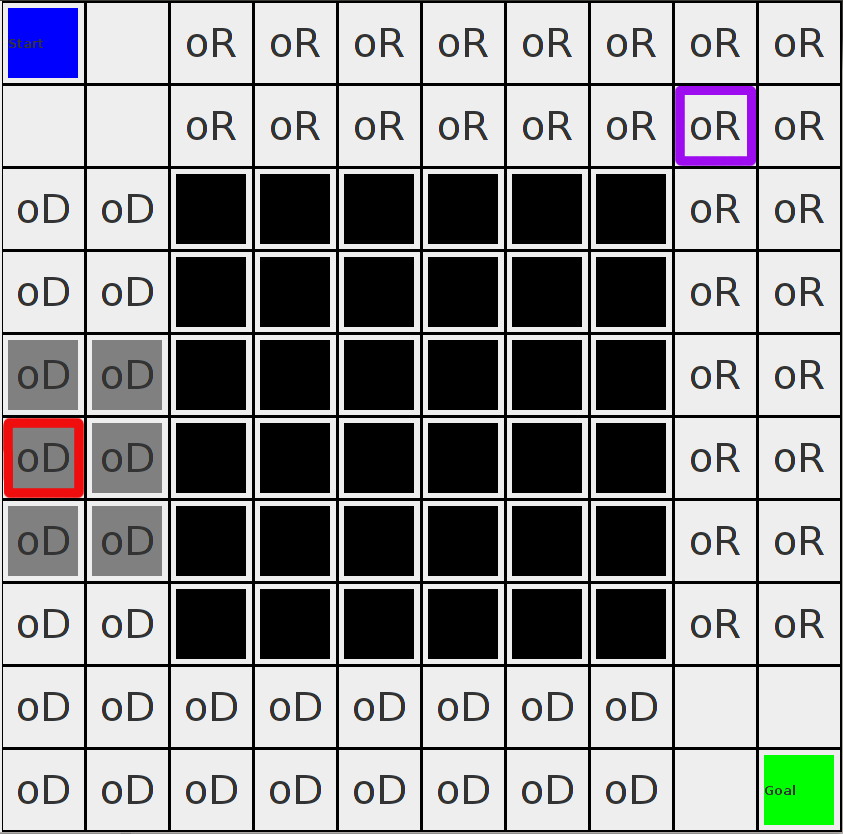
\includegraphics[width=2in]{ops.png}
    \caption{Environment with square obstacle, and two large options leading towards the goal (oD and oR). Blue square: start, Green square: Goal, Grey squares: interesting area, Purple outline: State 18, Red outline: State 50}
  \end{subfigure}\hfill
  \begin{subfigure}[h]{.45\textwidth}
  \centering
    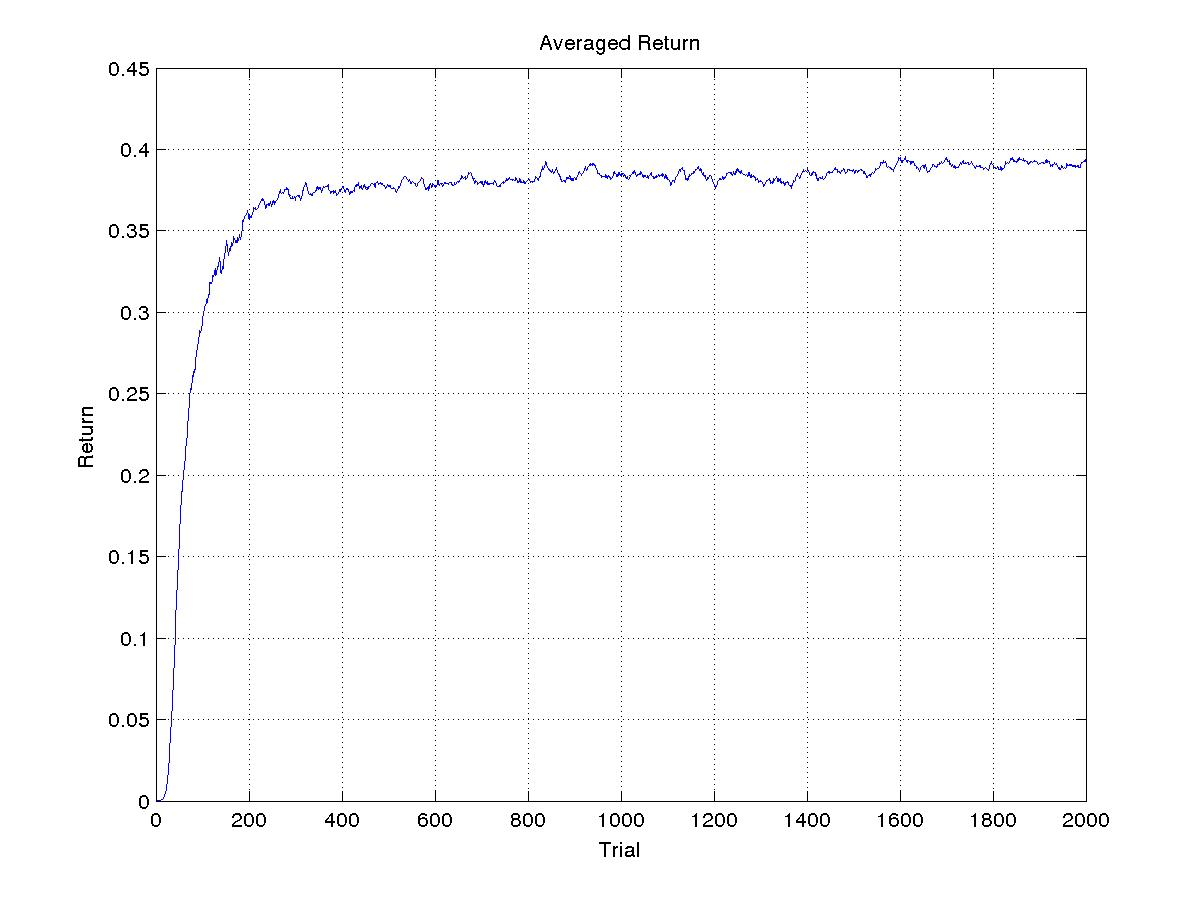
\includegraphics[width=3.5in]{return.jpeg}
    \caption{Average return accumulated over time, with error bars showing the standard error at each time step}
  \end{subfigure}
  \hfill
  \begin{subfigure}[h]{.45\textwidth}
  \centering
    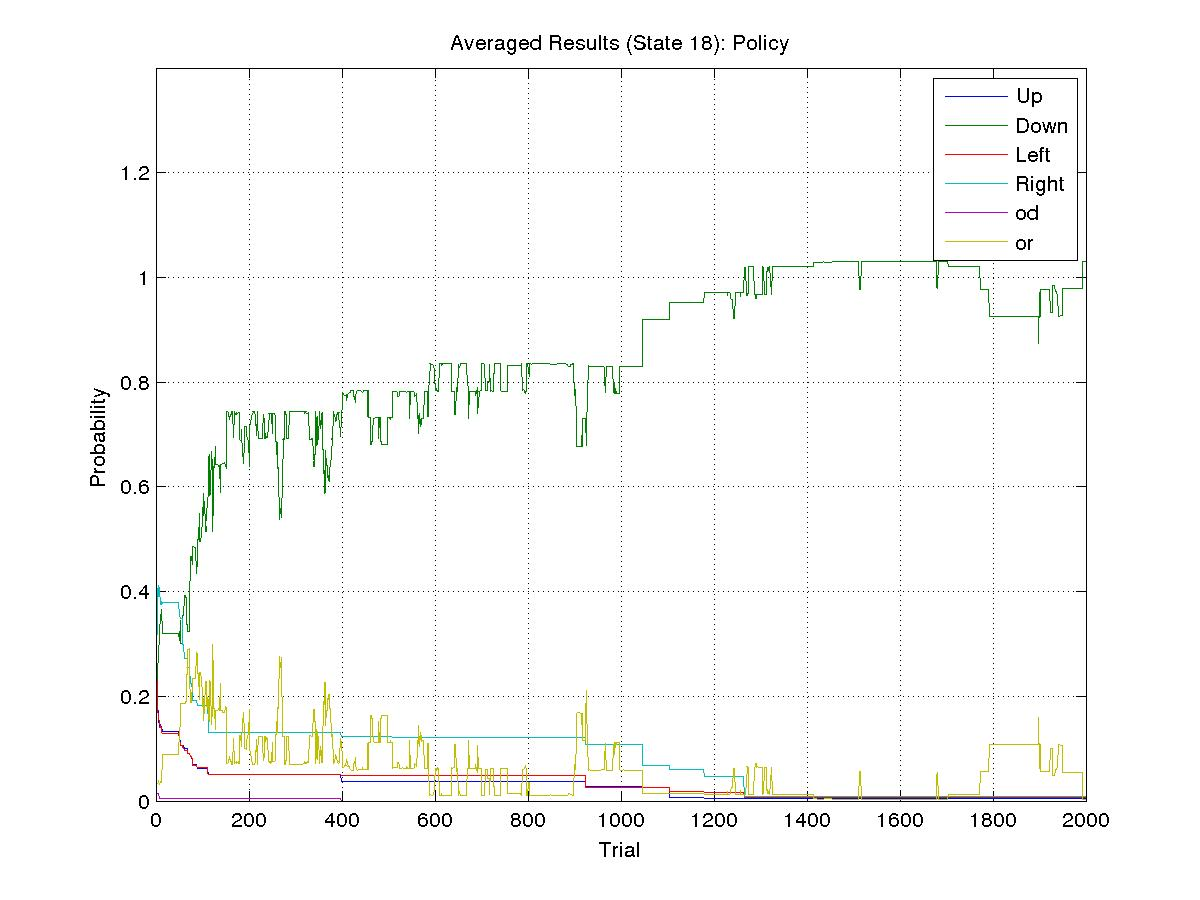
\includegraphics[width=3.5in]{pol18.jpeg}
    \caption{Policy over time at state 18. Green line: Probability of taking down action, Purple line: Probability of taking option oR}
  \end{subfigure}
  \hfill
  \begin{subfigure}[h]{.45\textwidth}
  \centering
    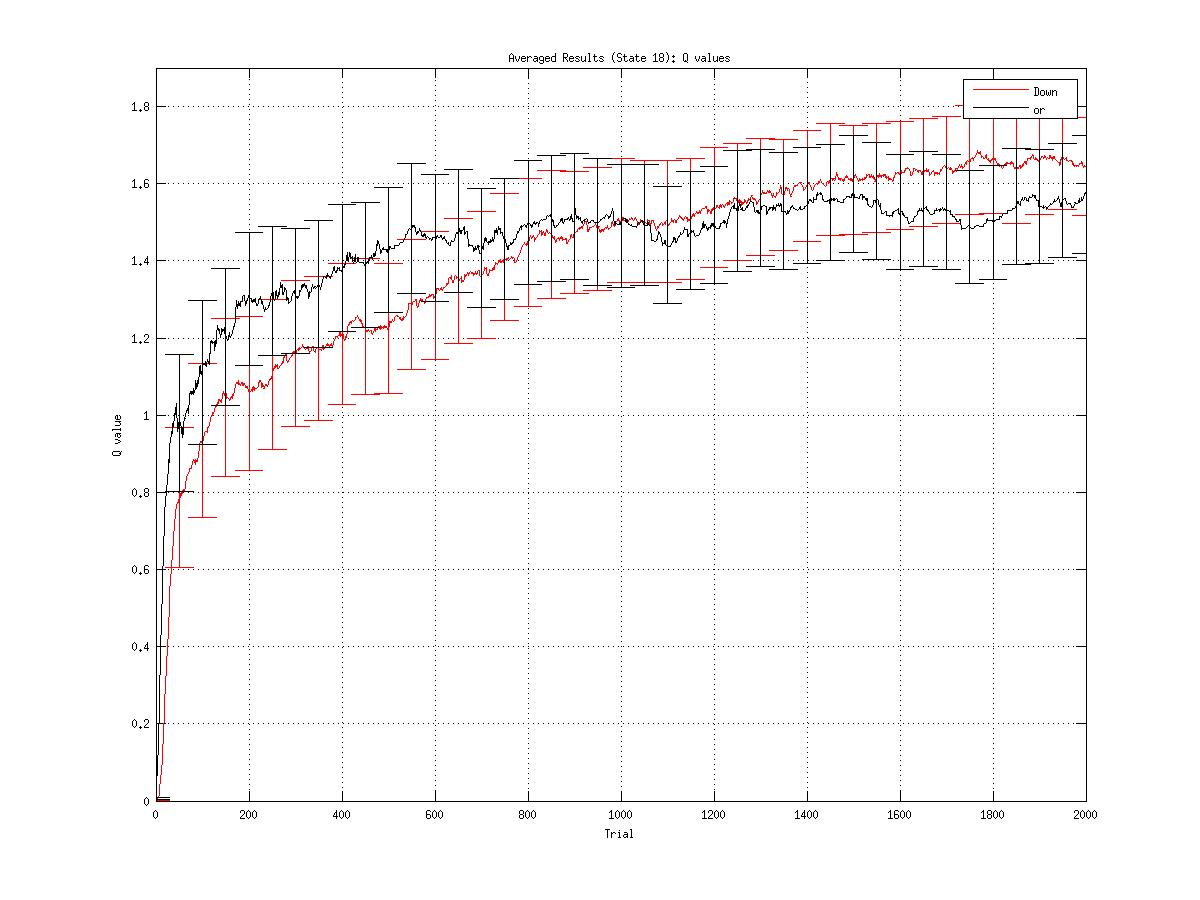
\includegraphics[width=3.5in]{Q18.jpeg}
    \caption{Q values over time at state 18. Red line: Q value for down action, Black line: Q value for option oR}
  \end{subfigure}
    \hfill
  \begin{subfigure}[h]{.45\textwidth}
  \centering
    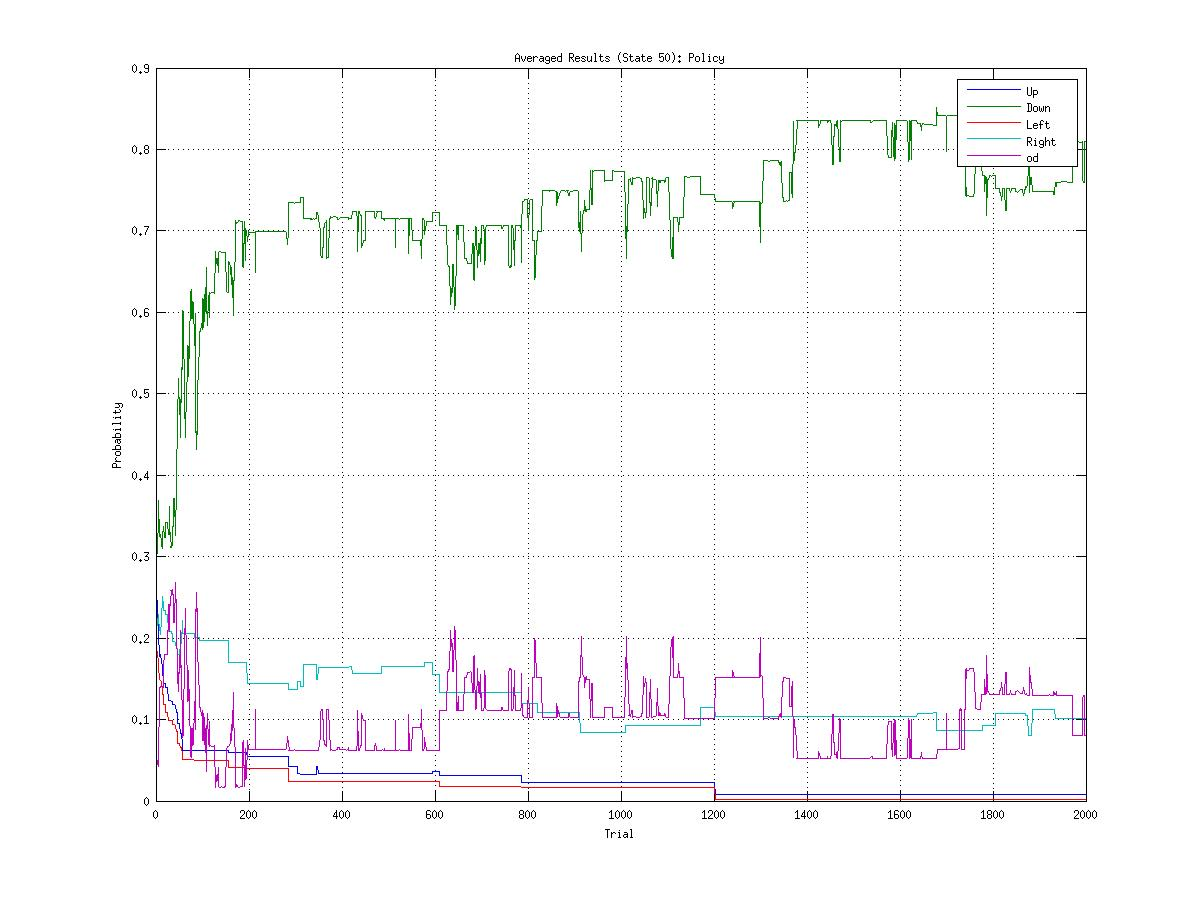
\includegraphics[width=3.5in]{pol50.jpeg}
    \caption{Policy over time at state 50. Green line: Probability of taking down action, Purple line: Probability of taking option oD}
  \end{subfigure}
    \hfill
  \begin{subfigure}[h]{.45\textwidth}
  \centering
    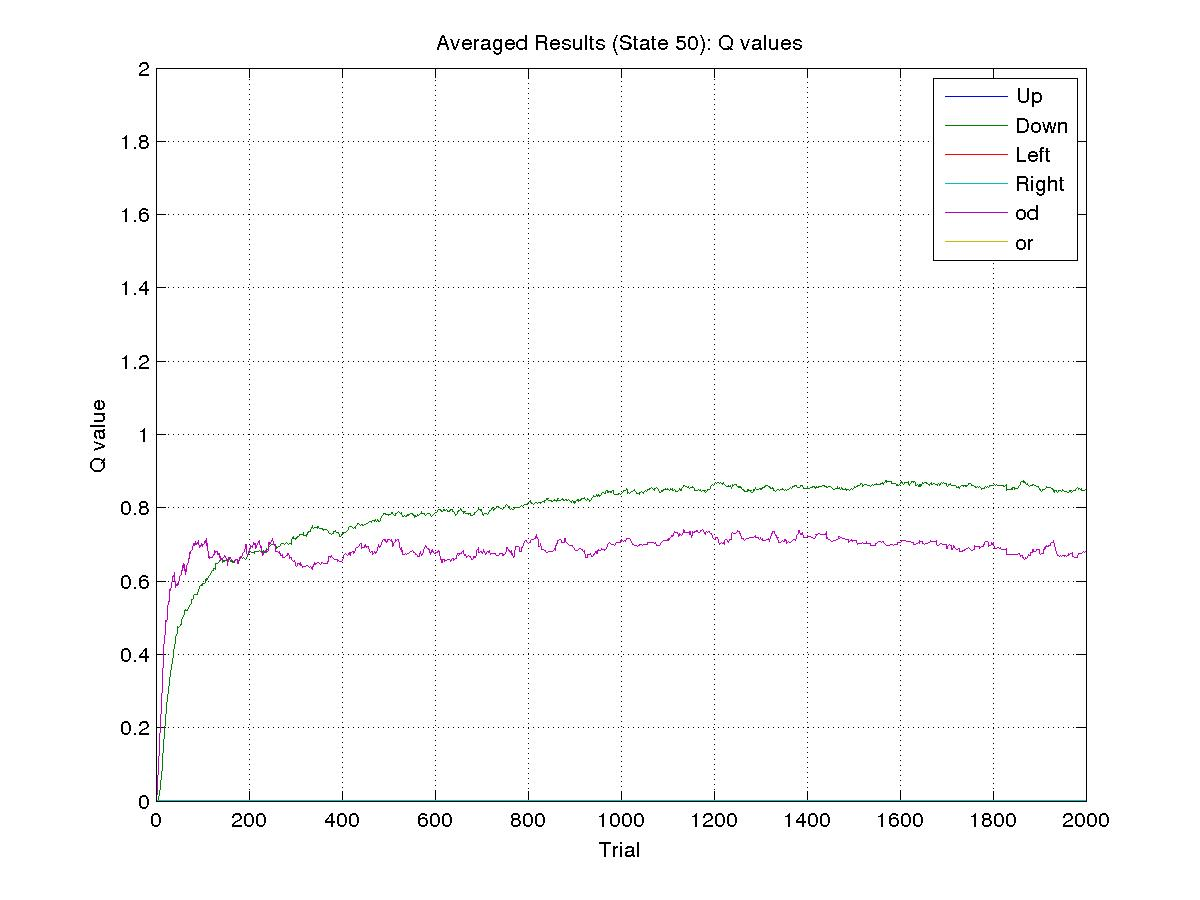
\includegraphics[width=3.5in]{Q50.jpeg}
    \caption{Q values over time at state 50. Red line: Q value for down action, Black line: Q value for option oD}
  \end{subfigure}
  \caption{Results of running the algorithm on an environment with one large obstacle and two hand-crafted options. The results are averaged over 20 full runs of the algorithm.}
  \vspace{20pt}
\end{figure*}

The goal of the next set of experiments was to determine whether eliminating options, which were not being used in the policy, during runtime would allow bad options to be eliminated early and good options to persist. 

For the first experiment we used the environment containing a large square obstacle, as previously described (see Figure 3(a)). However, in this case, 16 handcrafted options were evenly placed around the square obstacle, with four options having overlapping initiation sets on each side (see Figure 4(a)). Half of the options were considered "good" as they led the agent closer to the goal if taken, while the other half were considered as relatively bad since they would take the agent in the opposite direction. At each time step the agent would have to decide whether to keep or eliminate each of the options. Elimination in this case refers to complete removal of the option from all states. An option would only be removed if it was no longer being taken in any of the states in its initiation set (i.e. if the probability of choosing the option was less than 0.001 at any given state, as determined by the policy). 
	When observing only the order that options were removed, good and bad options appeared to be removed at random, with no clear preference for any specific option. However, after observing the number of states taking each option at each trial, it become evident that although the good options did not necessarily persist for much longer than the bad options, most states would stop using the bad options significantly earlier than the good ones. This therefore shows that the algorithm does in fact some way distinguish between options that it finds useful and ones that it finds less useful. 

%Sift
\begin{figure*}[!htbp]
	%\centering
  \begin{subfigure}[h]{.8\textwidth}
  	\centering
    \includegraphics[width=7in]{BlockEnv.png}
    \caption{Grid world with interesting area (Grey squares), obstacles (Black squares), and options (o1 - o16) shown. Blue square: Start, Green square: Goal}
  \end{subfigure}\hfill
  \begin{subfigure}[h]{.45\textwidth}
  \centering
    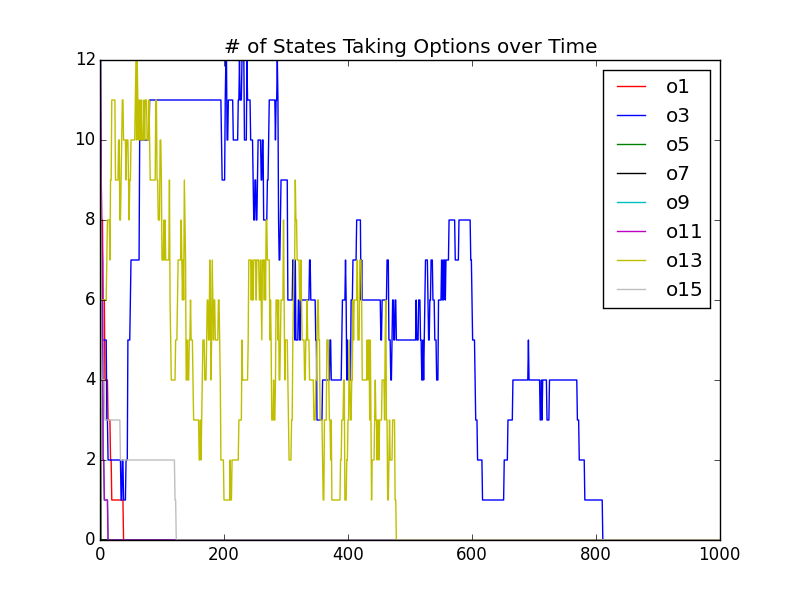
\includegraphics[width=3.5in]{good.png}
    \caption{Number of states taking each relatively good option over time}
    \end{subfigure}
  \hfill
  \begin{subfigure}[h]{.45\textwidth}
  \centering
    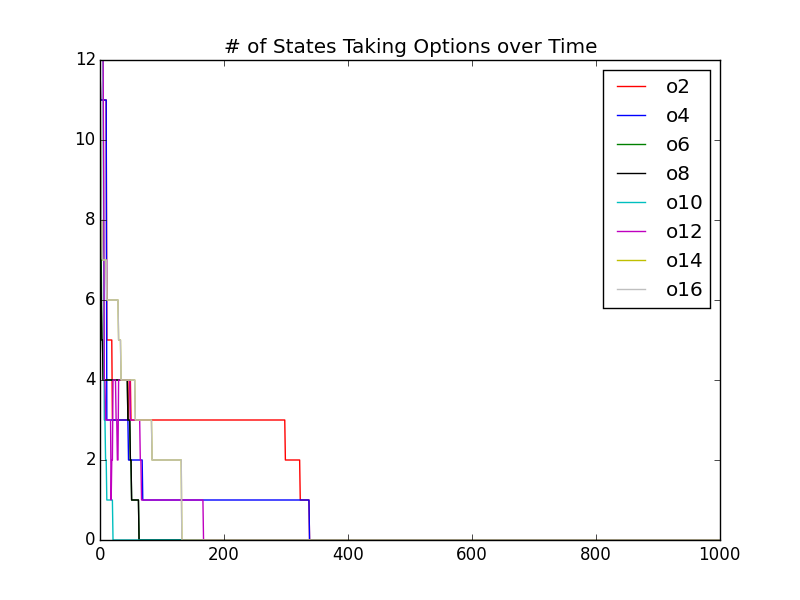
\includegraphics[width=3.5in]{bad.png}
    \caption{Number of states taking each relatively bad option over time}
  \end{subfigure}
  \caption{Results of experiment where algorithm sifts through 16 handcrafted options. Options are completely removed when the policy does not take the option with a probability > 0.001 in any of the states in its initiation set.}
  \vspace{20pt}
\end{figure*}

A different way to potentially find good options was also examined. Instead of using an all-or-none approach to remove options, here we tried a method which involved removing states from the options initiation set. If the option was no longer being taken at a certain state (i.e. the probability of taking the option was less than 0.0001), then that state was removed from the initiation set, thus shrinking the option, or even splitting it into two or more smaller options. 
	An obstacle-free grid environment was used, once again with a large random option consisting of all but one state. This was to help ensure that the final option(s) would be useable and not have an initiation set of simply one or two states. Furthermore, in order to prevent the primitive actions from overshadowing the option, as these are usually preferred, a penalty was placed on the action values of all primitive actions. More precisely, after each action value update for a primitive action, the action value would then be divided by 1.1, while the option's action values were not penalized. The results were promising as even options that were seemingly useless at first, mostly bringing the agent further from the goal, would eventually be trimmed into at least one useful option (see Figure 5). 

%Giant Sift
\begin{figure*}[!htbp]
  \begin{subfigure}[h]{.4\textwidth}
  	\centering
    \includegraphics[width=3in]{GiantSiftt3.png}
    \caption{Grey square represents the subgoal of the random option. Blue square: Start, Green square: Goal}
  \end{subfigure}\hfill
  \begin{subfigure}[h]{.4\textwidth}
  \centering
    \includegraphics[width=3in]{GiantSift3.png}
    \caption{Thick black arrows indicate states where option was taken, and the action corresponding to the options subpolicy at that state}
  \end{subfigure}
  \caption{Results of creating smaller options from a large random option. States were removed from the option's initiation set if the state would take the option with a probability < 0.0001. In (b), a darker red represents states that were visited more frequently.}
 % \vspace{20pt}
\end{figure*}

These combined results show support for the potential that this new method holds for a computationally efficient alternative for finding useful options. Although it does not perfectly discriminate between good and bad options, there is a clear preference for options that move the agent closer to the goal, and this preference oould be exploited to develop techniques to choose a decent set of options from a large random set. 

\section{Conclusions}

%Summarize results and there significance, talk about future work that could be done.

In reinforcement learning, the ability to create useful temporally extended actions programatically is important for many complex or large environments. Being able to do so efficiently is of equal importance, sometimes more so than the overall quality of the temporally extended actions created. Here we have proposed a novel method for generating options efficiently, without any prior knowledge of the environment or its dynamics required. Our results give support for a method in which several options are first generated randomly, and then sifted to determine those which are worth using in the given environment.   
	Although even good options were not frequently incorporated into the final policy found by the algorithm, our results suggest that this was simply due to the corresponding primitive actions being preferred, as can be seen in Figure 3. One possible solution to this issue was tested when we attempted to break up a large random option into potentially several smaller options (see Figure 5).
	%This could be seen when observing the action values in Figure 3 (d) and (f), where although the options initially showed higher action values, and the primitive action's action values gradually became higher over time.
	Here, we penalized the primitive actions to avoid the option being removed in states where it was beneficial. This technique worked relatively well in discovering at least one useful option of decent size, however; further testing of different techniques to penalize primitive actions may still be needed to optimize the results. 
	
	Our results also suggest an alternative to penalizing actions. Rather, one could remove unused options over time, and instead observe how rapidly an option is removed. In other words, by examining the number of the states taking the option over time. Based on our results, good options will be used by more states over a longer period of time when compared to bad options. However, only a set of handcrafted options was tested with this method, and further examination needs to be done to see whether it is plausible to use with random options.
	
	Finally, more work is still needed to see whether these methods would work well in different settings, and to compare them to other option finding algorithms. Furthermore, using different aspects of information theory, such as entropy instead of predictive information may be interesting to explore as well.	

%\end{document}  % This is where a 'short' article might terminate

%ACKNOWLEDGMENTS are optional
%\section{Acknowledgments}
%This section is optional; it is a location for you
%to acknowledge grants, funding, editing assistance and
%what have you.  In the present case, for example, the
%authors would like to thank Gerald Murray of ACM for
%his help in codifying this \textit{Author's Guide}
%and the \textbf{.cls} and \textbf{.tex} files that it describes.

%
% The following two commands are all you need in the
% initial runs of your .tex file to
% produce the bibliography for the citations in your paper.
\bibliographystyle{abbrv}
\bibliography{references}
\balancecolumns
% That's all folks!
\end{document}
